\question (中国科学技术大学,2004年)若一个有向图具有拓扑排序序列,那么它的邻接矩阵必定为(
)
\par\twoch{对称矩阵}{稀疏矩阵}{三角矩阵}{\textcolor{red}{一般矩阵}}
\begin{solution}一个有向图具有拓扑排序序列,说明它是个有向无环图(Directed Acyclic
Graph,简称DAG),但DAG图在邻接矩阵上没有直接的表示
\end{solution}
\question (北京航空航天大学,2004年)已知某有向图G=(V,E),其中V=\{v1,v2,v3,v4,v5,v6\},E=\{(v1,v2),(v1,v4),(v2,v6),(v3,v1),(v3,v4),(v4,v5),(v5,v2),(v5,v6)\},(
)是G的拓扑序列
\par\fourch{\textcolor{red}{v3,v1,v4,v5,v2,v6}}{v3,v4,v1,v5,v2,v6}{v1,v3,v4,v5,v2,v6}{v1,v4,v3,v5,v2,v6}
\begin{solution}画出下图即可求得G的拓扑序列。
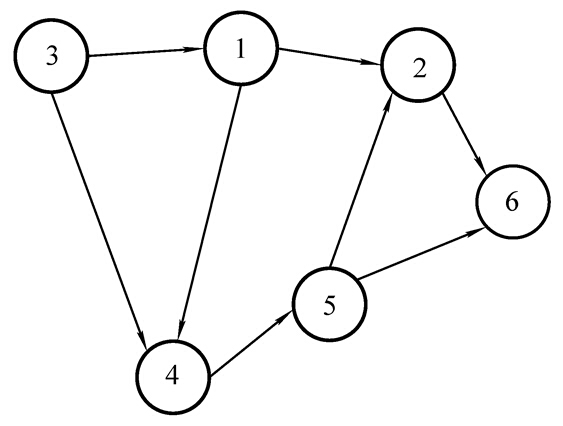
\includegraphics[width=2.08333in,height=2.08333in]{computerassets/81eae3ad3bd2585a68b0b81f131f8a7e.jpeg}
\end{solution}
\question (江苏大学,2006年)在有向图G的拓扑序列中,若顶点vi在顶点vj之前,则下列情形不可能出现的是(
)
\par\twoch{G中共有弧(vi,vj)}{G中有一条从vi到vj的路径}{G中没有弧(vi,vj)}{\textcolor{red}{G中有一条从vj到vi的路径}}
\begin{solution}如果vi在vj之前,则说明vi到vj一定有一条路径,而如果从vj也有一条路径到vi,则在该拓扑序列中存在一个环,这是不可能出现的,因此本题选D。
\end{solution}
\question 下列关于图的叙述,正确的是( )。 Ⅰ.回路是简单路径
Ⅱ.存储稀疏图,用邻接矩阵比邻接表更省空间
Ⅲ.若有向图中存在拓扑序列,则该图不存在回路
\par\twoch{仅Ⅱ}{仅Ⅰ、Ⅱ}{\textcolor{red}{仅Ⅲ}}{仅Ⅰ、Ⅲ}
\begin{solution}若路径中除了开始点和结束点可以相同以外,其余顶点均不相同,则称这条路径为简单路径。若一条路径中第一个顶点和最后一个顶点相同,则这条路径是一条回路(回路中可能存在既不是起点也不是终点的相同点),故Ⅰ错误。后话,要是两者是充要条件,也就不必要两个名词了。
邻接矩阵无论图是稀疏还是稠密,都取的是最大的存储空间,因此用邻接表比邻接矩阵更省空间,故Ⅱ错误。
用拓扑排序的方法可以判断图中是否存在回路,如果对一个图可以完成拓扑排序,则此图不存在回路,故Ⅲ正确。
【总结】
本题考查了图的多个知识点,但本题目出的不是很好,属于3个比较简单的判断题的生硬拼凑,不能算是好的``综合''题。但做题的同学需要掌握多个基础知识点才可正确解答。
\end{solution}
\question 对下图进行拓扑排序,可以得到不同拓扑序列的个数是( ~)。
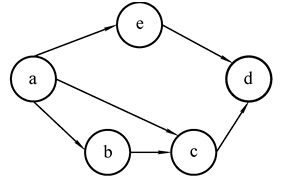
\includegraphics[width=2.93750in,height=1.87500in]{computerassets/47e0ad54c481720d18a9c25b7cc54696.jpeg}
\par\twoch{4}{\textcolor{red}{3}}{2}{1}
\begin{solution}拓扑排序的步骤为: ~ ~ ~
~(1)在有向图中选一个没有前驱的顶点并且输出之。 ~ ~ ~
~(2)从图中删除该顶点和所有以它为尾的弧。 ~ ~ ~
~(3)重复上述两步,直至全部顶点均已输出或图中剩余的顶点中都有前驱。后者说明有向图中有环。
~ ~ ~
~由于没有前驱的顶点可能不唯一,所以拓扑排序的结果也不唯一。解题过程如下图所示:
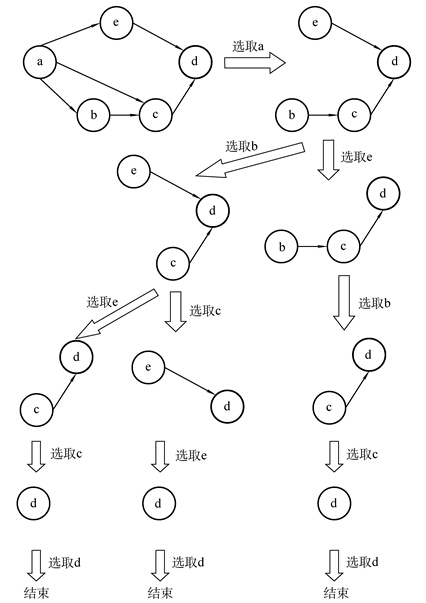
\includegraphics[width=3.33333in,height=4.71875in]{computerassets/b2de19171affe09b50c14eeca59f9f21.jpeg}

故本题有3个不同的拓扑排序序列,分别为:abced、abecd、aebcd。 【总结】 ~
~ ~ ~本题属于很基本的拓扑排序题目,知道基本的拓扑排序步骤即可顺利求解。
\end{solution}
\question (武汉大学,2004年)如果有向图中的顶点不能排成一个拓扑有序序列,则可以判定图中(
)
\par\twoch{顶点与顶点之间的关系太复杂}{边的数目为0}{\textcolor{red}{含有顶点数目大于1的强连通分量}}{有多个入度为0的顶点}
\begin{solution}如果不能排成一个拓扑有序序列,则证明一定有环出现,即一定含有顶点数目大于1的连通分量
\end{solution}
\question (中山大学,2004年)下图为AOE网,则可能的拓扑有序序列为( )
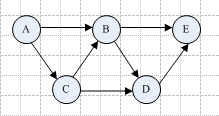
\includegraphics[width=2.28125in,height=1.20833in]{computerassets/0b432eb3cfa59d0b9d8b2ba6bab1eba5.png}
\par\twoch{ABDCE}{ABCDE}{\textcolor{red}{ACBDE}}{ACDBE}
\begin{solution}按照拓扑排序的步骤,只有C答案符合
\end{solution}
\question (北京交通大学,2004年)下图中有向图的所有拓扑序列有( ~)个
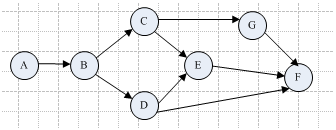
\includegraphics[width=3.33333in,height=1.29167in]{computerassets/13B306A6FB077FB89E8953D9BB02AF06.png}
\par\twoch{4}{\textcolor{red}{5}}{6}{7}
\begin{solution}拓扑排序的过程中选取入度为0的节点有多种情况,因此能得到多个不同的拓扑排序序列,一共有5种,ABCGDEF、ABCDEGF、ABCDGEF、ABDCGEF、ABDCEGF
\end{solution}
